\chapter{Udviklingsmodel - Scrum}
Under dette projektforløb er scrum udviklingsmodellen brugt til processtyring. Denne udviklingsmodel er en iterativ metode der bruges til styring, organisering og planlægning af produkt udviklingen.

%I dette afsnit beskrives den udviklingsmodel der anvendes i forbindelse projektets forløb. I dette projekt er der blevet gjort brug af scrum som udviklingsmetode.

\section{Rollebeskrivelser}
Der er tre hovedroller i scrum; produktejeren, udviklingsholdet og scrum masteren. Disse tre roller udgør scrum teamet. Under dette projekt har gruppevejlederen fungeret som produktejeren, udviklingsholdet har bestået af projekt gruppen og rollen som scrum masteren er skiftevis varetaget af forskellige medlemmer af gruppen.

\subsection{Produktejer}
Når der udvikles et produkt er der som regel en produktejer, der har stor interesse i det endelige produkt. Produktejeren definerer rammerne omkring produktet og prioriterer vigtigheden af opgaver på backloggen. \newline

I dette projektforløb er rollen som produktejer en kunstig rolle, i den forstand at gruppen har sat rammerne omkring projektet og prioriterer opgaver under forløbet. Gruppens vejleder har påtaget sig rollen som produktejer, men har meget lidt indflydelse på udkommet af projektet. Til sprintenes afslutnings møder fungerede vejlederen som en konventionel produktejer. Her blev resultaterne af sprintet fremført for produktejeren, som skulle forholde sig kritisk i forhold til resultaterne.

Under et sprintplanlægningsmøde havde produktejeren en reel indfyldelse på prioritering af opgaver, og opgaverne på sprintbackloggen. Inden mødet med produktejeren havde gruppen afholdt et møde og udvalgt de vigtigste opgaver til sprintet. Herefter blev mødet med produktejeren afholdt, som hjalp med prioriteringen af opgaverne og gav foreslag til opgaver, der ikke var taget højde for.  

\subsection{Udviklingshold}
Udviklingsholdet består af en gruppe individer, der arbejder mod et samlet mål; et færdigt delprodukt for hvert sprint. Udviklingsholdet er selvorganiserende, dermed udpeges der ikke nogen holdleder. \newline

I dette projekt bestod udviklingsholdet af projektets gruppemedlemmer, der hver især har forskellige egenskaber, der giver værdi til holdet. Det er udenfor normerne at scrum masteren er en del af udviklingsholdet. Dette er dog tilfældet under dette projektforløb, da det ville hindre projektet at udelade en person fra udviklingsholdet på grund af sin rolle som scrum master. \par
Under førløbet har udviklingsholdet været mere eller mindre selv organiseret. Der er dog nogle deadlines og krav, der skulle overholdes fra IHA's side.


\subsection{Scrum master}
En af hovedrollerne i scrum er scrum masteren. Scrum masterens vigtigste rolle er at sikre at processen i projektforløbet er bevaret. Med dette menes at scrum masteren skal sørge for at udviklingsholdet overholder reglerne for scrum ved at coache dem i at anvende scrum. Derudover skal scrum masteren fungere som bindeled mellem produktejeren og udviklingsholdet. Der er mange andre vigtige opgaver som scrum masteren typisk skal varetage sig, så som ordstyrer til daglige morgenmøder, hjælpe holdet med at afgøre hvad der skal udføres i et sprint og holde et alment overblik over gruppens fremskridt. Da scrum i dette tilfælde anvendes til et semesterprojekt og ikke et fuldtidprojekt, er der nogle dele af scrum master rollen vi har taget til os, nogle som vi anvender på vores egen måde og nogle som vi ser bort fra. \newline

Under dette projekt overtog et nyt gruppemedlem rollen som scrum master for hvert sprint. Som scrum master havde man to ansvarsområder; holde overblik over logbøgerne og fungere som bindeled mellem produktejeren og udviklingsholdet. \newline

En central rolle for scrum-masteren er at være ordstyrer for de daglige stå-op-møder, samt at sørge for at skaffe hjælp til udviklingsteamet når der opstod problemer. Det er ikke scrum masteren ikke noget ansvar til at løse problemerne, men derimod er scrum masteren med til at afhjælpe problemet ved at gøre resten af gruppen opmærksom på de nyopstandne problemer, eller at skaffe hjælp udefra. 

Som bindeled skulle scrum masteren kommunikere med produktejeren, som i dette tilfælde var gruppens vejleder. Til sprintplanlægningsmøder skulle gruppen bestemme hvad der skulle foretage i det næste sprint. Ved rigtig anvendelse af scrum ville produktejeren være til stede til disse møder for at få afstemt forventninger omkring det næste sprint. Derefter ville scrum masteren, med produktejerens ønsker i tankerne, sætte opgaver på sprintbackloggen sammen med udviklingsholdet. Da dette ville være en tidskrævende process, blev det bestemt at vejlederens tilstedeværelse ikke var nødvendig til denne process og blev først konsulteret efter backloggen var blevet udfyldt med opgaver. Til møderne fungerede scrum masteren som ordstyrer og oprettede opgaver på Pivitol Tracker efter gruppens ønsker. \par 
Under forløbet er gruppens dokumenter til dokumentationsrapporten blevet reviewet af en anden gruppe. Her skulle scrum masteren samle dokumenterne, der skulle reviewes, og lave mødeindkaldelser til reviewmøderne.





\chapter{Projektgennemførsel}

Følgende afsnit beskriver essentielle \textit{ting} som blev gjort brug af til at gennemføre projektet. 

% \section{Gruppedannelse}


\section{Samarbejdsaftale}
For at få et godt projekt, og en god oplevelse i projektgruppen, blev der udarbejdet en samarbejdskontrakt. Denne indeholder after iforhold til forventning af mødedeltagelse, gruppeledelse, og ambitioner for selve projektet. Samarbejdsaftalen kan ses bilaget.

%En samarbejdsaftale er god til at få skabt et fælles grundlag for forventninger og ambitioner til et projektforløb. Som indledning til arbejdet og udviklingen af dette projekt blev der udfærdiget en samarbejdskontrakt, som tog afsæt i en tidligere benyttet aftale, som nogle af gruppens medlemmer anvendte i forbindelse med forrige semesterprojekt. Den var velstruktureret og havde fungeret godt, og den var derfor et godt udgangspunkt for samarbejdskontrakten til dette projekt. Fokus i aftalen er på forventninger til mødedeltagelse, gruppeledelse og ambitioner for selve projektet. I forhold til gruppeledelsen er personligt ansvar og fælles forpligtelse vægtet højt. Udgangspunktet var, at en koordinator stod for sekretæropgaver og for at holde overblik, men at den egentlige ledelse med tillid og ansvar blev pålagt gruppens medlemmer i fællesskab. Tidligt i projektforløbet blev der indført Scrum som udviklingsmodel, og dermed blev koordinatoren erstattet med en scrummaster, som faciliterede udviklingen. Den fælles forpligtelse og det overordnede ansvar lå stadig hos de enkelte gruppemedlemmer.

\section{Arbejdsfordeling}
%\textbf{Der skal måske bare laves en tabel til at beskrive det her} \\
Som udgangspunkt blev gruppen opdelt i to hovedgrupper; en softwaregruppe bestående af Mia, Michael, Kasper, Tenna og Daniel, og en hardwaregruppe bestående af Mikkel og Pernille. Denne inddeling skete på baggrund af studieretning og dermed som resultat af interesser og kompetencer. På trods af den indledende opdeling i hardware og software, som tog udgangspunkt i erfaring og interesser, gav arbejdsfordelingen, stadig store muligheder for at blive udfordret, da flere af opgaverne skulle løses inden den relaterede undervisning havde været afholdt. I tilfælde hvor der opstod problemer, var opdelingen ikke mere fast, end at gruppens medlemmer kunne hjælpe hinanden på tværs af de tildelte opgaver. \\

% \section{Planlægning}
% Er blevet skrevet meget om i forvejen

\section{Projektledelse}
Scrum er en udviklingsmodel der ikke understøtter en projektleder i en traditionel forstand. Der har dog for hvert sprint været en ny scrum master, der skulle holde overblik over processen og gruppens medlemmer. Under dette projektforløb har der været brug for en til at styre opgaver som sekretær og mødeleder. Derfor forekom det naturligt gruppen at scrum masteren overtog dette ansvar udover sin rolle som scrum master. Det har været scrummasterens opgave at have kontakt til vejleder, at lave dagsorden til møderne og indkalde til disse. Da gruppen er selvorganiserende og påtager ansvar for egne opgaver, har der ikke været en decideret projektleder, som har uddelegeret opgaver. 
% I dette projekt er projektledelse anvendt på den måde, at der i hvert sprint har været en ny scrummaster, som har fungeret som en slags sekretær for gruppen. Det har været scrummasterens opgave at have kontakt til vejleder, at lave dagsorden til møderne og indkalde til disse. Dermed har der været meget fokus på fælles forpligtelse i forhold til, at alle gruppemedlemmer har haft ansvar for, at deres egne opgaver blev udført til tiden, så der ikke har været en decideret projektleder, som har uddelegeret opgaver. Det har gruppen stået for i fællesskab, hvilket også har virket meget tilfredsstillende. 

\section{Møder}
Gennem hele projektforløbet har der været afholdt et ugentligt vejledermøde. Dette møde har undertiden været brugt til at afholde review- og retrospective-møder i forbindelse med scrum. Det er til hvert vejledermøde tilstræbt at der blev udarbejdet en dagsorden, som kunne bruges som udgangspunkt for referatet af mødet. På hvert møde blev det aftalt, hvornår det næste vejledermøde skulle afholdes. Scrummasteren sørgede for at indkalde til disse møder via mail til vejleder og over Facebook til resten af gruppen. 

Udover de ugentlige vejledermøder er der blevet afholdt interne møder i gruppen, når det har været nødvendigt. Disse blev der indkaldt til over Facebook, så alle gruppemedlemmer var klar over, at de blev afholdt. Disse møder blev afholdt efter behov, og der var altså ikke et fast antal møder om ugen. 

En central del af scrum, er de daglige stå-op-møder. Disse har været en udfordring for os at holde, idét at vi har haft forskellige mødetider i løbet af dagen. For at løse dette problem har vi prøvet flere alternativer. Først prøvede vi at bruge logbøger, hvor scrum-masteren havde til opgave at kigge logbøgerne igennem for eventuelle råb om hjælp. I logbøgerne skulle følgende spørgsmål besvares:

\begin{itemize}
	\item Hvad lavede du i går?
	\item Hvad skal du lave i dag?
	\item Skal der bruges hjælp?
\end{itemize} 

Vi fandt dog ud af, at logbøgerne ikke var en god måde for os at afholde vores daglige stå-op-møde, idét det var et stort arbejde for alle at finde ud af hvad den enkelte havde lavet. Efter at have prøvet logbøgerne i et stykke tid, prøvede vi at holde "ordentlige" stå-op-møder i en uge. Dette holdt vi op med igen, da vi ikke kunne få det til at hænge sammen med vores skemaer. Som et sidste alternativ, prøvede vi at oprette en facebook samtale hvor alle gruppemedlemmer var indblandede. I denne samtale blev der hver morgen skrevet hvad man havde lavet i projektet, samt hvad man havde planlagt at arbejde videre med, samt fremhæve evt. problemer man var stødt på. Denne måde at holde stå-op-møde på, har fungeret bedst for vores gruppe, idét at man hurtigt og let får et overblik over hvad de andre gruppemedlemmer arbejder med, og eventuelle problemer de måtte have.

\section{Projektadministration}
Under dette projekt er der anvendt nogle værktøjer til administrere projektet. Disse værktøjer er alle internetbaseret da disse skulle være lettilgængelige for alle gruppemedlemmer og kunne anvendes på trods af manglende faste grupperum.

\subsection{GitHub}
Her skriver Kasper noget om GitHub og fællesfildeling. 
Rieder er en ho

\subsection{Pivotal Tracker}
For at have et scrum board på nettet, som alle kunne tilgå blev Pivotal Tracker anvendt. Pivotal Tracker er et professionelt scrum værktøj, der indeholder mange funktioner blandt andet scrum boardet, grafer og statistikker. Programmet blev valgt ud fra en anbefaling fra vores vejleder.

\textbf{Der skal billeder ind af sprintlog eller lignende} 

\subsection{Facebook}
Til kommunikation mellem gruppensmedlemmer blev der oprettet en Facebook gruppe. Denne gruppe blev brugt til lave aftaler, fildeling og almen kommunikation. Dette værktøj var en essentiel del af gruppe kommunikationen da det er noget som bruges i dagligdagen og det var et værktøj man i forvejen havde kendskab til. \newline

Da der skulle aftales arbejdsdage for påsken blev der oprettet en afstemmning. Med denne afstemmning fik hver medlem tilkendegivet hvilke dage de havde til rådighed. Resultatet af afstemmningen var de to dage der havde størst opbakning. Dette ses i figur \ref{ref:fbpoll}, som er et udsnit af afstemningen.
\begin{figure}[H]
	\centering
	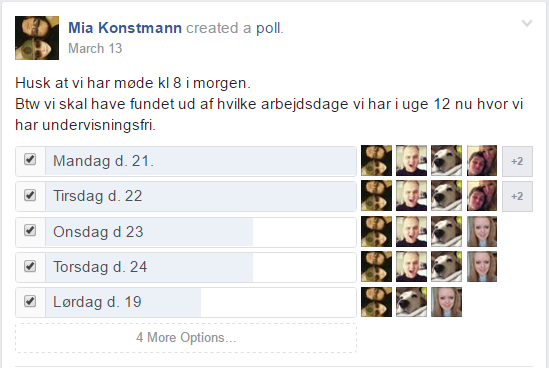
\includegraphics[scale=0.6]{Projektgennemfoerelse/images/fbpoll}
	\caption{Afstemning omkring arbejdsdage}
	\label{ref:fbpoll}
\end{figure}

Facebook gruppen fungerede som en opslagstavle, hvor der kunne dele informationer og meddele hinanden omkring hvordan dokumentation skulle håndteres. Under dette projekt er der blevet brugt LateX til dokumentation. Dermed skulle der lave aftaler omkring hvordan referencer skulle håndteres når det afsnit man refererede til endnu ikke var skrevet. På figur \ref{ref:fblatex} ses at løsningen til dette problem beskrives med en vejledning omkring hvordan referencer skal håndteres.

\begin{figure}[H]
	\centering
	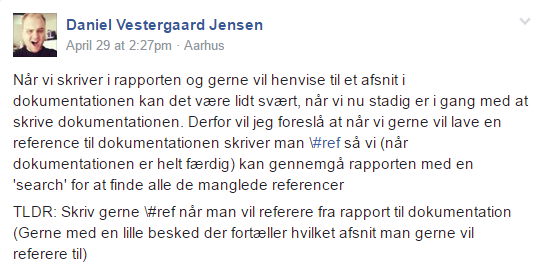
\includegraphics[scale=0.6]{Projektgennemfoerelse/images/fblatex}
	\caption{Opslag omkring referencer}
	\label{ref:fblatex}
\end{figure}

Til at erstatte stå op møderne og logbøger er der blevet oprettet en gruppesamtale. I denne chat informerede man hinanden omkring det der var foretaget dagen før og det der skulle foretages på dagen. Et udsnit af denne samtale ses på figur \ref{ref:fbchat}. Denne form for kommunikation fungerede bedre end de andre forsøg der var blevet gjort i forgående sprint. 

\begin{figure}[H]
	\centering
	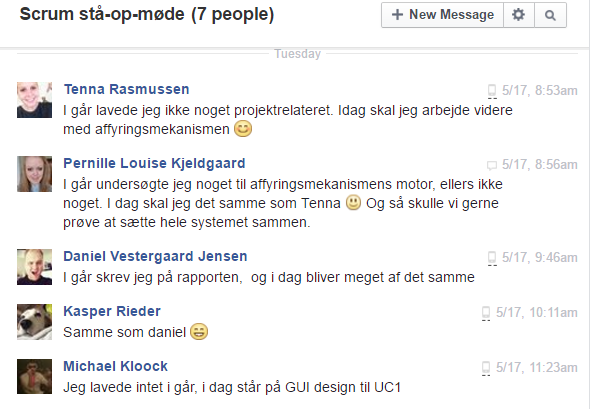
\includegraphics[scale=0.6]{Projektgennemfoerelse/images/fbstandup}
	\caption{Udsnit af gruppesamtalen}
	\label{ref:fbchat}
\end{figure}

Til dette projekt har Facebook været et vigtigt kommunikationsværktøj. Det blev muligt for gruppens medlemmer at kommunikere med hinanden på trods af varierende undervisningstimer og personlige skemaer. Ved at bruge Facebook påmindede man hinanden om at opretholde kommunikationen når man fik en notifikation på sin startside.

\chapter{Scrumkursus ved Systematic}
Som en del af projektet deltog gruppens medlemmer i et scrumkursus som udbydes af Systematic. Som udgangspunkt havde gruppen arbejdet med scrum i to måneder inden kursets start, dermed var der en forforståelse af hvordan scrum skulle anvendes i forbindelse med projekt arbejde. I de følgende afsnit vil de erfaringer som gruppen har gjort sig under kurset.

\section{Planning Poker}
En af øvelserne til kurset var planning poker. Her var opgaven at planlægge en flytning, hvor handlingerne for at nå målet skulle tidsestimeres. Under denne øvelse konstaterede gruppen at der var stor uenighed om hvor meget tid der skulle sættes af for at udføre hver delopgave. Der var nogle medlemmer som var optimistiske og forventede at opgaver var hurtigt overstået uden nogle hindringer. Mens der var nogle medlemmer der var pessimistiske og forventede at noget kunne gå galt under udførelsen af opgaverne, som ville forårsage tidsspild. En af opgaverne der skulle planlægges, hvor gruppen var meget uenige i tidsestimeringen, var en teoretisk opgave omkring klargøre et værelse til flytning. Under denne øvelse fik gruppen diskuteret begrundelserne for deres tidsestimeringer og dermed har gruppen fået erfaringer med en alternativ måde at tidsestimere på. Planning Poker er dog ikke blevet brugt under dette projekt forløb, men det har givet værktøjer til at organisere selve tidsestimerings processen.

\section{Scrum Spillet}
En anden af øvelserne til kurset var scrum spillet. Her blev gruppen præsenteret med en backlog af små, veldefineret opgaver. Hver af disse opgaver havde en pointværdi. Når en opgave var fuldført og godkendt af produktejeren, kunne gruppen lægge denne pointværdi til den totale pointsum. Der blev udført tre sprint hver på 15 minutter. Før hvert sprint var der et sprintplanlægningsmøde på 10 minutter og efter hvert sprint var der aflagt fem minutter til retrospective. \newline

Under sprint planlægningsmøderne valgte gruppen de opgaver, som skulle laves i sprintet. Disse kunne enten udføres individuelt eller i grupper, og hvert gruppemedlem meldte sig selv ind på de opgaver de følte de kunne udføre. Dette betød også at hver medlem havde ansvar for de opgaver, som man havde sat sig på og dermed var der en forpligtelse til at udføre opgaven før sprintets afslutning. \newline

Under sprintene var der meget samarbejde omkring arbejdsopgaverne. Når et gruppemedlem konstaterede at der ikke var nok tid til at fuldføre en opgave, blev der hurtigt set på hvilke medlemmer der kunne assistere. Her var gruppen god til at holde overblik og være selvorganiserende. Dette skyldes at kommunikationen fungerede. I modsætning til projektarbejdet, skulle der ikke ydes en indsats for at kommunikere med gruppens medlemmer, da de var omkring en selv. 
I og med opgaverne var veldefinerede, skete der sjældent misforståelser omkring opgavens natur, hvilket betød at arbejdet kunne startes hurtigt. Når der var tvivl omkring opgaverne kunne man konsultere en produktejer som opklarede tvivlen med en klar melding, som gruppen kunne forholde sig til og rette sig efter.  \newline

Til retrospective fik gruppen talt om hvad der fungerede og hvad der ikke fungerede for sprintet. Under første sprint var der ingen struktur omkring hvordan backloggen var sorteret og hvor sprintopgaverne var placeret, hvilket skabte forvirring når der var pres på under selve sprintet. Herefter blev der opsat en struktur i form af lommer der var katagoriseret i \textit{Udførte opgaver} og \textit{Backlog}. I Udførte lommen lå godkendte opgaver og i Backlog så de opgaver der endnu ikke var påbegyndt. Disse opgaver var sorteret, så hurtige og lette opgaver lå øverst og kunne tages hvis der ikke var flere opgaver på sprintbackloggen. De sprintopgaver man havde ansvar på fik man i hånden, så man kunne give den til produktejeren når der skulle godkendes en opgave. \newline
Denne øvelse gav os erfaring med, hvor vigtigt det er at have et organiseret arbejdsrum, og veldefinerede opgaver i forbindelse med scrum og sprints.

\section{Perspektivering}
Under dette kursus har gruppen fået en praktisk forståelse omkring brugen af scrum. Vi oplevede at kommunikationen mellem gruppens medlemmer lykkedes, når vi er fysisk tilstede og har en fysisk og veldefineret sprintbacklog, som vi kan forholde os til. Det ville derfor gavne gruppen at have et grupperum hvor et fysisk scrumboard kunne sættes op. Dermed får vi muligheden for at visualisere de opgaver, der skal udføres i sprintet. \newline
I modsætning til projektarbejdet, var der en ansvarsfølelse for de opgaver der skulle udføres i sprintet. Dette skyldes at vi til scrum spillet valgte opgaver efter vores egne evner og med en sikkerhed om at man kan fuldføre opgaven. Til projektet er arbejdsopgaver valgt med usikkerhed da projektets opgaver omhandler noget man ikke nødvendigvis har kendskab til og er en del af en læringsprocess.

\chapter{Udviklingsforløb}
I de følgende afsnit vil udviklingsforløbet af projektet beskrives for hvert sprint. Herunder vil der de erfaringer der blev gjort for hvert sprint beskrives.

	\section{Sprint 1}
	\textbf{19/2/16 - 14/3/16}\newline
	\textbf{Varighed:} 3 uger\newline
	\textbf{Scrum master: }Kasper \newline \newline
	Formålet med det første sprint var at dokumentere, implementere og teste use case 2, Test Kommunikationsprotokoller.
	Sprintet startede ud med at lave en backlog i Pivotal Tracker. Der blev lavet userstories på baggrund af brugerønsker samt userstories til de dokumenter, der udgør de tre færdige rapporter. Herefter blev to userstories udvalgt til sprint backloggen, der skulle arbejdes på i dette sprint. Disse userstories består af underopgaver, der hørte til implementeringen af hardware og software. Når en underopgave blev færdiggjort, blev den krydset af i userstory'en. \newline
	
	I kravspecifikationen blev det bestemt der skulle anvendes tre PSoC til I2C kommunikationen mellem GUI, motor og nunchuck. Under arkitektur dannelsen så vi at PSoC2 forbundet til nunchucken kun pollede for information og videredesendte det. Ved at fjerne PSoC2 forbundet til nunchuck'en og forbinde den til PSoC1 forbundet til motoren. Dermed overtager PSoC1 funktionaliteten af PSoC2 og vi undgår unødig kommunikation. \newline
	
	Under sprintet udførte vi diverse opgaver, der ikke stod i sprint backloggen. Dette blev gjort da vi havde glemt at definere dem som userstories da vi udvalgt opgaver til sprintbackloggen. Dermed er der blevet udført meget mere under sprintet end der kan ses på Pivotal Tracker. \newline
	
	Under dette sprint har vi anvendt logbøger, i stedet for daglig stand up møder. Der blev hver morgen noteret det, som man egentligt ville have nævnt til de daglige møder. Det gav en del arbejde til scrum masteren, der skulle tjekke hver dag om alle havde lavet dagens indlæg. Derudover forsvandt kommunikationen mellem gruppensmedlemmer i perioder, da der ikke var nogen andre end scrum masteren, der kiggede logbøgerne igennem. Dette gav anledning til en del miskommunikation omkring arbejdsdage og arbejdsopgaver. For at undgå dette vil vi forsøge os med daglige stand up møder, med vejlederen, i næste sprint. \newline
	
	\begin{figure}[H]
		\centering
		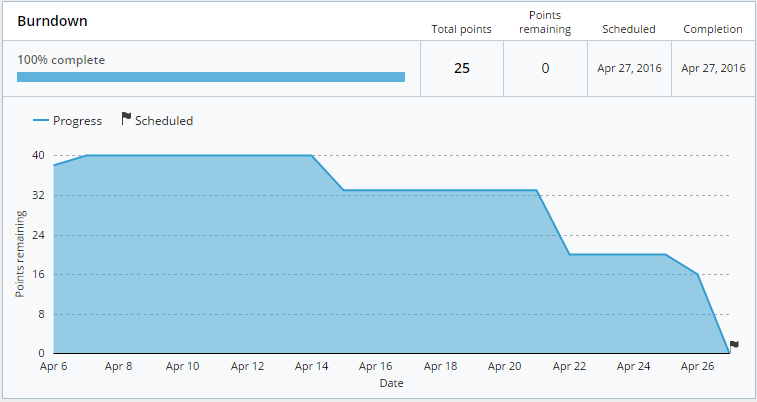
\includegraphics[width=\textwidth]{Projektgennemfoerelse/images/burndown1}
		\caption{Burndown chart for sprint 1}
		\label{ref:Burndown1}
	\end{figure}
	
	På figur \ref{ref:Burndown1} ses et burndown chart for første sprint. Dette billede er taget efter sprintet er afsluttet og derfor ser det ud til at 100\% af opgaverne er færdiggjorte. Ved at se på grafen kan man se at lige  inden sprintet afsluttede manglede der 16 point på sprintbackloggen. Grafen er præget af en plateau effekt. Dette skyldes størrelsen på opgaverne på sprintbackloggen. Det ser ud til at der er inaktive perioder efterfulgt af et dyk. Da vi ikke færdiggjorde nogen af vores userstories til fulde, medførte det at vi tilsyneladende ikke har opnået nogen resultater i dette sprint.  \newline
	
	\textbf{Under dette sprint har vi lært:}
	\begin{itemize}
		\item At user stories skal være mere findelt, for at kunne vise udviklingen af projektet
		\item At strukturen for PSoC opsætningen ikke var hensigtsmæssig, da PSoC1 kunne overtage funktionaliteten af PSoC2
		\item At vi skal holde os til sprint backloggen og kun arbejde på de opgaver vi har defineret for sprintet
		\item At der skal bruges mere tid til at opdatere gruppens status
	\end{itemize}
	
	Da sprintet var færdig er vi gået tilbage og ændret på sprint backloggen for både at findele de userstories vi havde inkluderet og for at dokumentere de ting der er blevet udført i dette sprint, som ikke var inkluderet. Derudover tager den erfaring vi har fået med arkitekturen med til et af de næste sprint hvor use case 2 skal implementeres. Da vi ikke havde så meget erfaring med scrum mistede vi under sprintet overblikket og dermed kom vi for langsomt i gang med implementeringen. Dette skyldes både vores uerfarenhed med scrum og dårlig tidsestimering. Vi opnåede meget i dette sprint, dog opnåede vi ikke det ønskede mål, som var en færdig implementeret use case 2. 
	
	
	
	\section{Sprint 2}
	\textbf{16/3/16 - 6/4/16}\newline
	\textbf{Varighed:} 3 uger\newline	
	\textbf{Scrum master: }Pernille \newline
	Formålet med anden sprint var at designe og implementere software og hardware til use case 2, Test Kommunikationsprotokoller. Sprintet startede ud med sprintplanlægningsmøde. Her blev der i gruppen blev aftalt hvilke userstories skulle laves under sprintet. Da disse var fastlagt blev der aftalt et sprintplanlægningsmøde med vejlederen, der hjalp med tidsestimering af disse opgaver. Dette var en langsommelig process, men dette var nødvendigt da vi ikke havde anvendt Pivotal Tracker ordentligt og havde problemer med tidsestimering i sidste sprint. Under mødet blev opgaverne også prioriteret, noget som ikke blev gjort i sidste sprint, dermed blev der skabt et overblik af de vigtigste opgaver til sprintet. \newline
	
	Som noget nyt forsøgte gruppen sig med stand up meetings. Dette var et forsøg på at anvende scrum i et større omfang end vi tidligere har gjort. I en hel uge blev der afholdt morgen møder med vejlederen inden dagens lektioner. Til disse møder blev der nævnt hvad man ellers ville have været skrevet i logbøgerne. Dette gjorde arbejdet lettere for scrum masteren, da hun skulle fungere som ordstyrer til disse møder, i stedet for at læse logbøger. Møderne gav gruppens medlemmer et overblik som man ikke havde fået ved logbøgerne, da man ikke aktivt skulle opsøge information omkring hvad de andre medlemmer foretog sig. Gruppen oplevede, at fordi vi havde kontakt med vejlederen dagligt, fik vi hurtig respons til opstandne problemer og hjælpen var bedre end det vi kunne modtage fra en mail. Der var dog nogle problemer med møderne, da den uge de kørte over, var en uge hvor der skete meget samarbejde. Dermed blev møderne en samtale omkring hvad hardware- og softwaregruppen havde lavet dagen forinden. Stå op møderne ville have fungeret meget bedre hvis de havde foregået i en uge hvor der blev arbejdet mere individuelt. \newline
	
	En af grundene til at opgaverne fra sprint backloggen ikke var fuldført var fordi at der i midten af dette sprint var påske ferie. Dette gav anledning til diskussioner i gruppen da der ikke var enighed omkring antallet af arbejdstimer i ferien. Løsningen på dette var at der blev aftalt to arbejdsdage i ferien, hvor der skulle arbejdes på projektet. Resten af ferien var det op til hver gruppemedlem at bestemme hvilke dage der skulle arbejdes. \newline
	
	\begin{figure}[H]
		\centering
		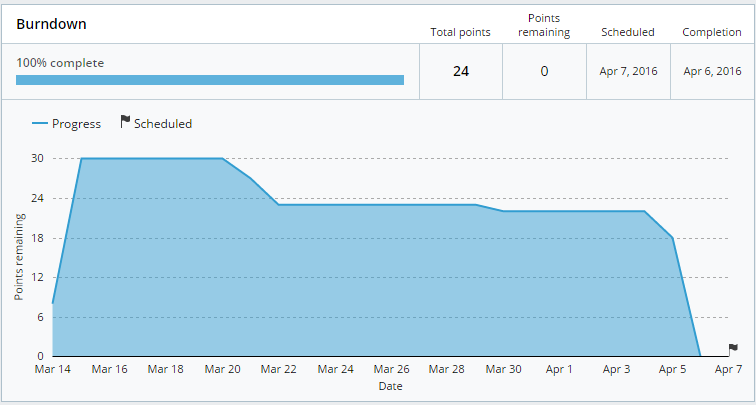
\includegraphics[width=\textwidth]{Projektgennemfoerelse/images/burndown2}
		\caption{Burndown chart for sprint 2}
		\label{ref:Burndown2}
	\end{figure}
	
	På figur \ref{ref:Burndown2} ses anden sprints burndown chart. Her ses at ved sprint afslutningen var der stadig 18 point i ufærdige opgaver på sprintbackloggen. Det ses også at sprintet blev afsluttet en dag tidligere end forventet. Grafen er stadig præget af en plateau effekt. Denne gang er det i en værre grad end ved første sprint. Dette skyldes formenligt flere dages inaktivitet under ferien og problemer med kommunikationsprotokoller i software. \newline 

	\textbf{Under dette sprint har vi lært:}
	\begin{itemize}
		\item At give opgaver realistiske tidsestimater
		\item At prioritere opgaver i backloggen
		\item At stå op møder fungerer ikke optimalt når der sker meget samarbejde
		\item At der skal bruges mere indsats for at kommunikere med gruppen 
	\end{itemize}
	
	Under dette sprint havde gruppen mere erfaring med scrum og anvendelsen af Pivotal Tracker end vi havde tidligere. Eftersom gruppen har arbejdet sammen i et længere stykke tid sker der færrer miskommunikationer. Da der stadig er problemer med tidsestimeringen blev backloggen ikke tømt for opgaver, men vi er kommet længere end forrig sprint. Målet for dette sprint er ikke opnået, men der er blevet udført nok til at vi føler at sprintet var vellykket.
	
	\section{Sprint 3}
	\textbf{7/4/16 - 27/4/16}\newline
	\textbf{Varighed: }3 uger \newline
	\textbf{Scrum master: }Mia \newline \newline
	Formålet med tredje sprint var at færdiggøre use case 2, samt få implemeteret dele af hardware til use case 1. Til sprintplanlægningsmødet oplevede gruppen et stort mandefald, da nogle af gruppens medlemmer var syge. Dette hindrede resten af gruppen i at planlægge sprintet efter alles ønsker. Da der var nogle medlemmer, som var dukket op på trods af sygdom, havde et ønske at tage hjem inden dagens lektioner blev dette møde timeboxed til en time. Under denne time fik gruppen fastlagt målet for sprintet og defineret de opgaver der skulle til for at nå dette mål. Da alle gruppens medlemmer ikke var til stede og der var sat den nødvendige tid af til sprintplanlægningsmødet oplevede vi igen at opgaverne ikke var veldefinerede og der var opgaver der manglede på sprint backloggen. \newline
	
	Under dette sprint deltog alle gruppens medlemmer i et scrumkursus som Systematic udbyder. Da scrum er den udviklingsmodel som anvendes til dette projekt, forekom det naturligt for gruppens deltagere at deltage som en gruppe. Hermed kunne de erfaringer og konklusioner som blev draget til kurset blive anvendt til at styrke gruppens kommunikation og samarbejde. 
	Til kurset blev der undervist i omfattende teori omkring scrum, der blev afholdt diskussioner og scrum blev taget i brug gennem øvelser. Øvelserne fokuserede på at træne evner, som har afgørende betydning for scrum. Disse inkluderede tidsestimering, planlægning, kommunikation og organisering. \newline
	
	Kommunikation er afgørende når der arbejdes med scrum. Dette noget vi oplevede da arbejdede med øvelserne til scrumkurset og da vi så på arbejdsgangen på Systematic. Gruppen har indset at logbøgerne, som blev genoptaget efter det fejlede forsøg med fysiske stand up meetings, ikke fungerede i en grad til at de kunne erstatte de fysiske stand up meetings, som scrum kræver. Kommunikationen i gruppen er ikke optimal, da der arbejdes mere individulet end der er blevet gjort hidtil, og der sker ingen kommunikation på tværs af undergrupperne. Derfor oprettes der en Facebook samtale, som skal sørge for kommunikationen. Med dette anvendes en platform som gruppen i forvejen bruger i dagligdagen til at opretholde kommunikationen.  \newline 
	
	\begin{figure}[H]
		\centering
		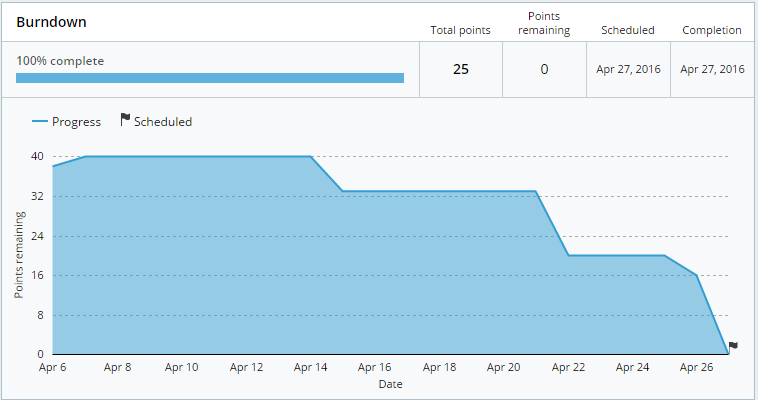
\includegraphics[width=\textwidth]{Projektgennemfoerelse/images/burndown3}
		\caption{Burndown chart for sprint 3}
		\label{ref:Burndown3}
	\end{figure}
	
	På figur \ref{ref:Burndown3} ses burndown chartet for sprint 3. Under dette sprint var opgaverne delt fint op, men det ses i figuren at der stadig er en plateau effekt. Dette skyldes at der var stor afhængighed mellem mange af de små opgaver. Det betød at der skulle meget forarbejde til at løse en opgave, men når denne så var færdiggjort, kunne andre opgaver hurtigt krydses af. Ved sprintafslutning stod vi tilbage med 16 point på backloggen. Dette skyldes at der var lagt op til mange rapportskrivnings opgaver, som var påbegyndt, men vurderet for udfærdig til at blive krydset af. \newline
	
	\textbf{Under dette sprint har vi lært:}
	\begin{itemize}
		\item At der skal sættes den nødevendige tid af til afholde sprintplanlægsningsmødet
		\item Hvordan scrum fungerer i praksis i forbindelse med en arbejdsplads
		\item At der fortsat skal ydes en større indsats for at kommunikere i gruppen
	\end{itemize}
	
	Under dette sprint opnåede gruppen sit sprintmål, som var færdiggørelse af use case 2. Alt software og hardware, der skal til, for at kunne udføre use case 2 er færdig implementeret og implementation for dele af hardware til use case 1 er påbegyndt. I dette sprint fik gruppen mulighed for at arbejde intensivt med scrum og kunne tage disse erfaringer med til selve projektet. 

	\section{Sprint 4}
	\textbf{27/4/16 - 18/5/16}\newline
	\textbf{Varighed: }3 uger \newline
	\textbf{Scrum master: }Tenna \newline \newline
	Formålet med fjerde og sidste sprint var at afslutte alle påbegyndte implementationsopgaver og starte på rapportskrivning. Da sprintbackloggen tidligere har været præget af problemer med tidsestimering skete der en taktik ændring til sprintplanlægningsmødet. Der blev set på hvor mange timer der var til rådighed for projektarbejde og lagde alle mandetimerne sammen. Herefter definerede vi time antallene for store, mellem og små opgaver, henholdsvis over 12 timer, 12 timer og 4 timer. Herefter blev der sat opgaver på sprintbackloggen indtil alle mandetimerne var afsat på disse opgaver. Dette resulterede i det største antal point på sprintbackloggen, i forhold til de forgående sprint.

	\begin{figure}[H]
		\centering
		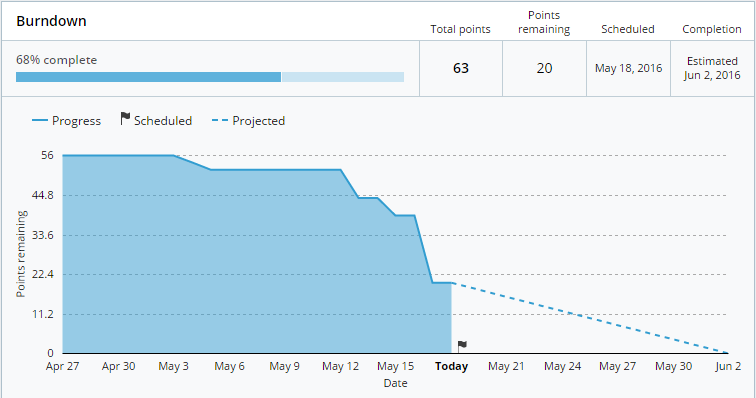
\includegraphics[width=\textwidth]{Projektgennemfoerelse/images/burndown4}
		\caption{Burndown chart for sprint 4}
		\label{ref:Burndown4}
	\end{figure}
	
	På figur \ref{ref:Burndown4} ses et burndown chart til sprint 4. Dette billede blev taget lige inden sprintafslutning, hvor man kan ses projektion af hvornår sprintet forventes at være afsluttet med den hastighed der blev arbejdet med under sprintetet. Der ses at der er blevet lagt det højeste antal point på sprintbackloggen, men det kan også observeres at der ikke er lagt opgaver ind efterfølge sprintets start. \newline
	
	\textbf{Under dette sprint har vi lært:}
	\begin{itemize}
		\item At der skal arbejdes på vores tidsestimeringsevner
	\end{itemize}

	Til sprintets afslutning var alle implementeringsopgaver færdiggjorte og de 20 point tilbage på sprintbackloggen var ufærdige rapportskrivningsopgaver. Dermed er gruppen meget tilfreds med det resultat der er opnået ved sprintets afslutning.  
% \section{Konflikthåndtering}
% Skal måske skrives


% \chapter{Opnåede erfaringer}
\chapter{Udfordringer ved anvendelse af scrum}
I forbindelse med at det er første gang, vi anvender scrum til et semester projekt, er der dele af scrum som vi har haft udfordringer med at få inddraget i udviklingsprocessen, hvilket har hindret processen.

\section{Kommunikation}
En vigtig del af scrum er kommunikation. Da gruppen bestod af medlemmer fra forskellige studieretninger, var det ikke muligt at afholde daglige morgen møder, og dette var en stor hindring for kommunikationen. Gruppensmedlemmer havde ikke overblik over hvad der foregik end det man selv var i gang med. Som kommunikationsværktøj blev der oprettet en Facebook gruppe. Her kunne gruppens medlemmer aftale arbejdsdage og informere hinanden om vigtige ting. Dette værktøj blev ikke anvendt så godt som det kunne have gjort, dermed skete der en del miskommunikation omkring arbejdsdage og hvornår man skulle mødes. \par

\section{Organisering}
Det er ikke muligt for grupper på tredje semester at få et grupperum. Dette ville have gjort en del for kommunikationen at man havde et fælles møderum, hvor der kunne arbejdes og hvor scrumboardet kunne placeres. Da dette ikke var en mulighed blev scrumværktøjet Pivitol Tracker anvendt. Der var uklarhed om hvordan dette værktøj skulle anvendes og det tog et par sprint før dette blev afklaret. Her ville det have været en fordel at have et scrumboard med sticky notes, som man arbejder normalt i scrum, eller eventuelt at gøre brug af et mindre kompliceret værktøj til at holde et online scrum-board. Dette kunne for eksempel være Trello eller lignende. 

\section{Sprintbackloggen}
Anvendelsen af Pivotal Tracker's backlog gik galt fra starten, da der ikke blev lavet en veldefineret liste. For hvert sprint blev der lavet nye opgaver alt efter gruppens ønsker til det kommende sprint. Det at der ikke en veldefineret backlog betød at der ikke kunne udvælges opgaver derfra, da disse opgaver ført blev definieret da vi kom i tanke om dem. \par
Sprintplanlægningsmøderne var præget af en manglende struktur og der blev ikke aflagt nok tid til at afholde disse møder. Dette betød at opgaver ikke var veldefineret og disse blev ændret i løbet af sprintet, som er noget der ikke må ske når der køres et sprint. Udover at opgaverne ikke var veldefineret, var der opgaver der ikke var taget højde for. Dermed blev der arbejdet på opgaver, der ikke var på sprintbackloggen og tog tid væk fra de tidsestimerede opgaver. Dette førte til at alle opgaver op sprintbackloggen aldrig blev fuldtført og tidsplanen blev ved med at skride.  

\chapter{Perspektivering}
Processtyringen af dette projekt har været præget af en usikkerhed og uerfarenhed. Dette kan ses i de problemer der er blevet stødt på under projekt forløbet, som for eksempel manglende kommunikation, forhastede planlægningsmøder og fejl i tidsestimeringer. Dette har dog ikke hindret gruppen i at prøve sig frem med nye metoder for at afhjælpe disse problemer. 
For at forbedre kommunikationen mellem gruppens medlemmer blev der forsøgt med forskellige metoder som logbøgerne og morgenmøderne. Vi oplevede dog at dette først blev forbedret da Facebook samtalen blev indført. 
Dette kan 
Der findes utallige metoder til tidsestimering 

Her beskrives hvad der mangler i udviklingsprocessen, og hvad der kan gøres
fremover for at optimere udviklingsprocessen. 